%! Author = wolfram_e_laube
%! Date = 06.05.24

\item[(b)]
\subsection{Task (b): Sampling and Spectrum Analysis of $x[n]$}

\subsection{Problem Statement}
The task involves analyzing the effects of sampling the analog signal $x(t)$ with a defined spectrum $X(f)$ at a rate of 8 kHz, to produce the discrete-time signal $x[n]$. The goal is to illustrate the spectrum of $x[n]$ from $-f_s$ to $f_s$ and to identify the baseband, demonstrating the effects of sampling on the signal's frequency spectrum.

\subsection{Analysis}
\subsubsection{Sampling Process}
The sampling frequency $f_s = 8000 \, \text{Hz}$ dictates the intervals at which the continuous-time signal $x(t)$ is sampled, producing the discrete-time signal $x[n]$. According to the Nyquist-Shannon sampling theorem, to prevent aliasing, the original signal’s bandwidth should ideally be less than $f_s/2 = 4000 \, \text{Hz}$.

\subsubsection{Spectrum of $x[n]$}
Sampling in the time domain introduces periodicity in the frequency domain, causing the spectrum of $x(t)$, $X(f)$, to repeat every $f_s$ Hz. The spectrum of $x[n]$ is thus a tiled version of $X(f)$, extending infinitely, but practically visualized from $-f_s$ to $f_s$.

\subsubsection{Baseband Definition}
The baseband is typically defined as the primary spectrum range from $-f_s/2$ to $f_s/2$ where the original signal's characteristics are most accurately represented without the influence of aliasing.

\subsection{Mathematical Definitions}
The spectrum of $x[n]$ within one period is defined as:
$$
X(f) =
\begin{cases}
1 & \text{for } -5000 \leq f \leq -1000 \text{ and } 1000 \leq f \leq 5000 \\
-\frac{f}{1000} & \text{for } -1000 < f < 0 \\
\frac{f}{1000} & \text{for } 0 \leq f < 1000 \\
0 & \text{otherwise}
\end{cases}
$$
This spectrum is periodically replicated across the frequency axis due to the sampling process.

\subsection{Conclusion}
The visualization of the spectrum of $x[n]$ from $-f_s$ to $f_s$ effectively illustrates how the original spectrum $X(f)$ is replicated due to sampling. The spectrum plot highlights the baseband and demonstrates the influence of sampling on signal processing, emphasizing the need for careful consideration of the sampling rate relative to the signal’s bandwidth to avoid aliasing. This analysis is crucial in digital signal processing applications where accurate representation and reconstruction of signals are necessary.

\begin{figure}[h]
    \centering
    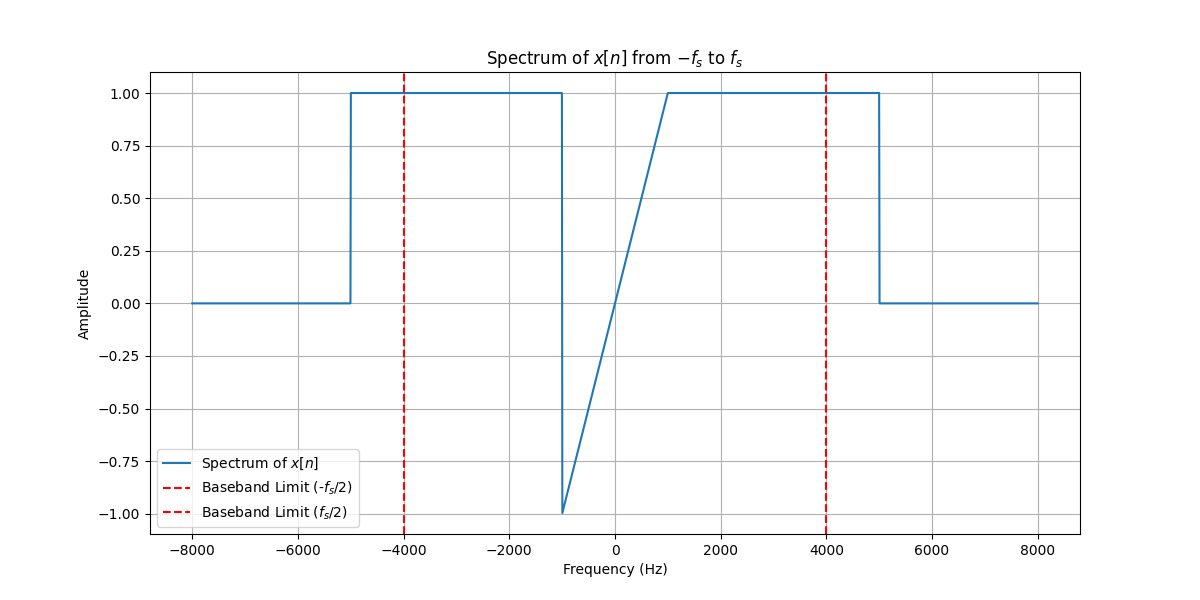
\includegraphics[width=0.49\textwidth]{fig/ex2_b_plot}
    \caption{Spectrum of \(x(t)\)}
    \label{fig:ex2_b_plot}
\end{figure}
